\expandafter\ifx\csname ifdraft\endcsname\relax
   \documentclass[a4j,12pt]{jsreport}
% 数式
\usepackage{amsmath,amsfonts}
\usepackage{bm}

% 画像
\usepackage[dvipdfmx]{graphicx}

% biblatex
\usepackage[style=numeric, sorting=none, maxbibnames=1000]{biblatex}
\addbibresource{graduation_thesis.bib}

%itembox
\usepackage{ascmac}
%breakitemboxのためのpackage
\usepackage{itembkbx}
% \usepackage{tcolorbox} 画像が見えなくなってしまう原因
% \usepackage{framed} 枠

%フォント
\usepackage[ipaex]{pxchfon}

\usepackage[top=35truemm,bottom=30truemm,left=30truemm,right=30truemm]{geometry}
\usepackage{float}
\usepackage{multicol}
\usepackage{paralist}
\usepackage{caption}
%\captionsetup{format=plain, justification=centering}
\usepackage{setspace}
\usepackage{algorithm}
\usepackage{algpseudocode}
\usepackage[dvipdfmx,hidelinks]{hyperref}
\usepackage{pxjahyper}
\usepackage{fancyhdr}
\usepackage{ltablex}
\usepackage{capt-of}
\usepackage{tabularx}
\usepackage{enumitem} % itemizeの行間 これは下になければならない
\usepackage{threeparttable} % 表の脚注
\usepackage{booktabs}
\usepackage{titlesec}
\titleformat{\chapter}[hang]{\LARGE\bfseries}{\prechaptername\thechapter\postchaptername}{1em}{}


   \setlength{\headheight}{16.5pt}
   \captionsetup{format=hang}
\begin{document}
% 上部のヘッダー
\pagestyle{fancy}
\lhead{\rightmark}
\renewcommand{\chaptermark}[1]{\markboth{第\ \thechapter\ 章\ #1}{}}
\fi

\chapter{Manga109ScriptDataset}\label{chap:proposedmethod}
本章では，本研究の第一段階において構築した，漫画画像に紐づく脚本データセットManga109ScriptDatasetについて，その構築手法や統計量，評価アノテーション手法の詳細を述べる．

序論で定義したとおり，本研究では漫画の「ネーム」を，幾何学的な「要素配置（Layout）」と「演出情報（Directions）」を統合した，物語と作品とを接続する中間表現として位置づける．このネーム生成に向けた取り組みに先立ち，第一段階では，物語としての「脚本」と「要素配置」との対応関係の学習に焦点を当て，Manga109ScriptDatasetを構築した．

構築においては，漫画画像を OpenAI API を介して GPT-4o に入力し，描画内容を脚本として記述させる手法を基本方針とした．本章では，この生成プロセスにおいて，モデルが複雑な文脈を正確に理解するために導入した画像加工やチャットフローの活用といった具体的な技術詳細について詳述する．

本章の構成は以下の通りである．まず~\ref{sec:dataset_design}節では，本データセットの基本設計として，対象データの概要および脚本形式の定義について述べる．続く~\ref{sec:visual_prompting}節では，LVLMのキャラクター認識精度の向上と，これに伴う正確な脚本生成を可能にするため実装したVisual Promptingについて述べる．\ref{sec:chat_flow}節では，画像間にまたがる連続的な文脈情報の理解を促進し，脚本内における物語の一貫性を確保することを目的に設計した，LVLMとのチャットフローについて示す．\ref{sec:statistics}節では，構築したデータセットの統計量を示し，最後に~\ref{sec:evaluation_data}節では，人手によるアノテーションに基づく脚本の品質評価手法と，その結果について論じる．

\section{本データセットの基本設計}\label{sec:dataset_design} 本節では，Manga109ScriptDatasetの構築において基盤となるManga109Datasetの選定理由および構築の対象とした記述フォーマットである脚本形式について述べる．

\subsection{Manga109Dataset}\label{sec:manga109} 　本研究では，漫画画像に対応する脚本生成の基盤データとして，Manga109Dataset~\cite{matsui2017sketch,aizawa_building_2020} を採用した，Manga109は，1970年代から2010年代に出版された日本の商業漫画109作品（計 21,142 ページ）から構成され，数多くの研究で取り上げられてきた\cite{}学術利用可能な漫画画像データセットである．少年漫画，少女漫画，青年漫画など多岐にわたるジャンルと画風を網羅しており，特定の作家やスタイルに過学習することなく，汎用的な漫画の構造を学習する上で最適なデータセットといえる．本研究では，Manga109に含まれる全作品を対象とし，見開き画像を片側単ページに分割した上で，表紙や広告などを除く計19,555ページに対して脚本データの構築を行った．Manga109Dataset内に含まれる画像の一例を図~\ref{fig:manga109example}に示す．

\begin{figure}[htbp]
   \centering
   \includegraphics[width=0.9\linewidth]{}
   \caption{Manga109Dataset に含まれる漫画画像の例}
   \label{fig:manga109example}
\end{figure}

\subsection{脚本形式} 　本研究において構築の対象とした物語文の形式は，日本の脚本形式に準拠する．脚本は映像制作現場において標準的に用いられる記述様式であり，テキストから視覚的イメージを具体化することを主目的として設計されている．その視覚化のための物語文というフォーマットは，ネーム生成というタスクにおいて親和性が高い．本研究では，Manga109が日本の漫画作品群であることを踏まえ，日本国内の制作様式において標準的に用いられている脚本形式をそのまま採用した．これは，将来的な制作支援応用を見据えた際，プロの作家や編集者が違和感なく扱える形式となるよう実応用性を考慮したためである，その形式は，以下の3つの主要な構成要素から成る．

\begin{enumerate}

   \item \textbf{柱}: 物語の場面転換を示すヘッダー情報．行頭に記号「◯」を付記し，その後に「場所」や「時間帯」を記述する（例：◯ 公園・昼）．

   \item \textbf{ト書き}:
         キャラクターの動作，表情，視線，および周囲の環境音や状況説明を記述する文章．視認性を高めるため，全角3文字分のインデント（字下げ）を行って記述する．これは，コマ割りや構図（カメラワーク）を示唆する重要な情報源となる．

   \item \textbf{セリフ}:
         キャラクターの発話内容．「話者名『セリフ内容』」の形式で記述する．
\end{enumerate}

本データセットの構築においては，漫画画像を入力とし，これらの構造化された物語文の構築を目指した．実際に生成された脚本の例を図~\ref{fig:script_example}に示す．

\section{Visual Prompting}\label{sec:visual_prompting}
本節では，LVLM の画像認識能力を補助し，正確な脚本生成を実現するために導入したVisual Prompting について述べる．

Manga109ScriptDataset の構築において，最も重要な要件の一つは，生成される脚本内で動作主や話者を正確に特定することである．しかし，第2章で述べた通り，漫画画像は白黒の線画表現であり、しばしばキャラクターが著しくデフォルメされるといった独自のドメイン特性を持つため，GPT-4o などの最新 LVLM であっても，そのまま適用するだけでは正確な認識，特にキャラクターの識別は十分になされない\cite{}．そこで本研究では，登場人物を取り違え，物語の整合性を著しく損なうハルシネーションを抑制するための手段として，画像内に視覚的な手がかりを直接埋め込む Visual Prompting を採用した．キャラクターの顔を色のついた円で囲い，視覚的な識別補助を与える手法である．

Manga109Dataset には，キャラクターの顔領域を示す Bounding Box が付与されており，各領域は作品内で一意のキャラクターIDと紐付いている．本研究ではこの情報を利用し，以下の手順で画像に加工を施した．まず，作品内に登場するキャラクターIDごとに，HSV色空間上で等間隔となるよう識別性の高い色を動的に割り当てる．次に，各顔領域に対して，割り当てた色で顔を囲う円を描画した．図\ref{fig:visual_prompting_example}に加工後の画像を示す．

\begin{figure}[htbp]
   \centering
   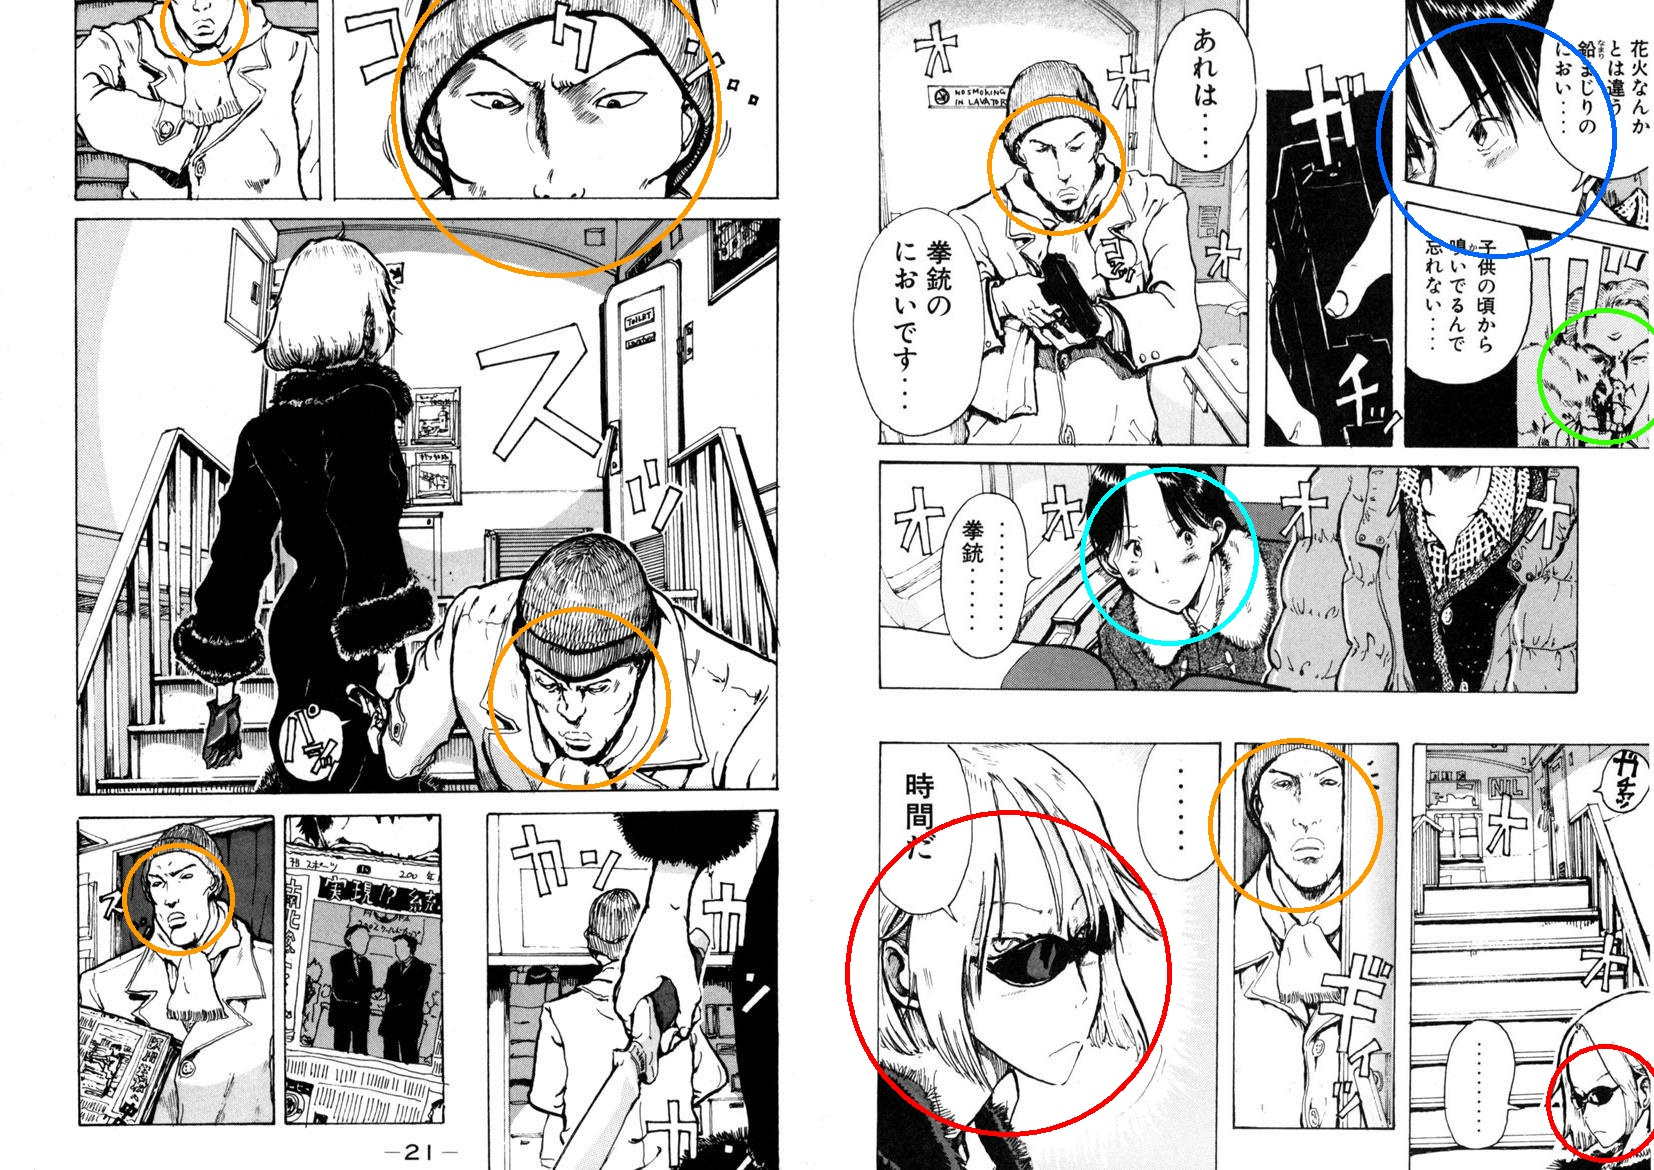
\includegraphics[width=0.9\linewidth]{pict/03/HanzeiKousyouninMinegishiEitarou10.jpg}
   \caption{Visual Prompting の例}
   \label{fig:visual_prompting_example}
\end{figure}

このアプローチは，Shtedritskiら~\cite{shtedritski_what_2023} の手法を漫画ドメイン向けに適応させたものである．この処理により，LVLM はデフォルメされた顔の識別といった高難度なタスクを色の識別という単純な視覚タスクへ置き換えることが可能となる．結果として，複雑な線画や類似したキャラクターが混在するシーンにおいても，モデルは視覚的アンカーを手がかりとして強固にキャラクターの識別能力を向上させた．

\section{画像間文脈理解のためのチャットフロー}\label{sec:chat_flow}
本節では，ページ間の文脈を考慮し，物語の一貫性を担保するために設計したチャットフローについて述べる．

\subsection{入力データの前処理と順序決定}
前節で述べた Visual Prompting に加え，モデルがキャラクターの同一性や会話の文脈を正しく理解するためには，正確なテキスト情報とその読み順が不可欠である．そこで本研究では，以下の2つの外部情報を利用し，漫画画像内の一連のセリフをプロンプト内で提示した．

\begin{enumerate}
   \item \textbf{テキストアノテーション}:
         各フキダシ内のテキスト内容および話者名については，Manga109Dialog~\cite{li_manga109dialog_2024} のアノテーションデータを使用．

   \item \textbf{読み順の決定（Magiアルゴリズム）}:
         コマやフキダシの読み順決定には，Sachdevaら~\cite{sachdeva_manga_2024} による Magi アルゴリズムを採用．
\end{enumerate}

ここで Magi を採用した理由は，LVLM 単体での空間的な順序推定能力の限界にある．我々の予備実験において，GPT-4oに画像のみを与えて読み順を推定させたところ，サンプリングした109ページ中，正解したのはわずか26ページに留まった．対照的に，ルールベースの手法である Magi を用いた場合，96ページにおいて正確な順序が得られた．この結果は，脚本生成の前段階として，アルゴリズムによる明示的な順序決定が不可欠であることを示している．

\subsection{文脈維持のための3段階インタラクション}
複数ページにわたる連続した物語を矛盾なく記述するため，本研究では GPT-4o に対して単純な1往復の指示を与えるのではなく，各ページ $i$ の生成において以下の3つのコンポーネント（$\alpha, \beta, \gamma$）から成る構造化されたインタラクションプロセスを構築した．

\begin{itemize}
   \item \textbf{$\alpha(i)$: 大域的文脈の理解 } \\
         ここでは，ページ単位の処理に入る前に，脚本生成の対象となるページ$i$が含まれるエピソード全体の一連のセリフをモデルに入力する．モデルからの応答を「完了」の肯定的応答としてシミュレートすることで，チャット内における文脈理解状態を確立させた．

   \item \textbf{$\beta(i)$: ページ $i$ の脚本生成 } \\
         実際に脚本を生成するフェーズである．入力として，「Visual Prompting を施したページ $i$ の画像」，「ページ $i$ のセリフテキスト」，および「直前のステップ $\gamma(i-1)$ で生成された物語の要約（Summary）」を与える．
         ここで過去の要約を与えることにより，モデルは「前ページまでの展開」を踏まえた上で，整合性の取れたト書きやセリフを脚本形式で生成することが可能となる．

   \item \textbf{$\gamma(i)$: 文脈情報の要約と更新 } \\
         次ページ $i+1$ の生成に備え，ここまでの物語の展開を要約させるフェーズである．生成された脚本と対話履歴に基づき，ストーリーの現状（誰がどこで何をしているか）を要約として出力させ，これを次のステップ $\beta(i+1)$ の入力として再利用する．
\end{itemize}

\subsection{シーケンスの実行}
本研究では，各ページ $i$ の脚本生成において，物語の一貫性を保持するために以下のシーケンスを実行した．ここで，矢印は同一チャットセッション内での対話の遷移を示している．

\begin{itemize}
   \item \textbf{先頭ページ ($i=1$) の場合} \\
         過去の文脈が存在しないため，以下の順序で実行する．
         \[
            \alpha(1) \rightarrow \beta(1)
         \]
   \item \textbf{第2ページ以降 ($i \ge 2$) の場合} \\
         直前のページの生成結果を履歴として保持しつつ，以下の順序で実行する．
         \[
            \alpha(i) \rightarrow \beta(i-1) \rightarrow \beta(i)
         \]
\end{itemize}
このように，脚本生成 $\beta(i \ge 2)$ においては常に一つ前のやり取りを履歴に残し，物語の一貫性を保持する工夫とした．また，次ページへの文脈受け渡し用として要約を生成する際は，以下のシーケンスへと拡張した．
\begin{itemize}
   \item \textbf{先頭ページ ($i=1$) の場合}
         \[
            \alpha(1) \rightarrow \beta(1) \rightarrow \gamma(1)
         \]
   \item \textbf{第2ページ以降 ($i \ge 2$) の場合}
         \[
            \alpha(i) \rightarrow \beta(i-1) \rightarrow \beta(i) \rightarrow \gamma(i)
         \]
\end{itemize}

各作品に対し，この一連のインタラクションを最終ページまで反復的に適用することで，Manga109ScriptDataset の全データを構築した．

\section{データセットの統計量}\label{sec:statistics} 　構築された Manga109ScriptDataset の詳細な統計量を表~\ref{tab:statistics} に示す． 　チャットフローを用いた生成の結果，109作品・計19,555ページに対し，約2万7千件の柱，約14万件のト書き，および約13万件のセリフを含む脚本データが構築された．

\begin{table}[htbp]
   \centering
   \setlength{\abovecaptionskip}{2pt}
   \caption{ Manga109ScriptDataset の統計量．「Distinct character types」はページごとのキャラクターIDのユニーク数，「Distinct speaker types」はページごとの話者IDのユニーク数を示す． }
   \label{tab:statistics}
   \begin{threeparttable}
      {\setlength{\tabcolsep}{5pt}
         \begin{tabular}{l r r}
            \toprule
            \textbf{要素}             & \textbf{総数}   & \textbf{平均 (/頁)} \\ \midrule
            \multicolumn{3}{l}{\textit{レイアウト要素 }}                      \\
            \hspace{0.5em}総ページ数     & 19{,}555      & \textemdash      \\
            \hspace{0.5em}コマ数       & 103{,}850     & 5.31             \\
            \hspace{0.5em}キャラクター検出数 & 157{,}865     & 8.70             \\
            \hspace{0.5em}キャラクター種類数 & 60{,}812      & 3.11             \\
            \hspace{0.5em}フキダシ数     & 146{,}549     & 7.49             \\
            \hspace{0.5em}話者種類数     & 55{,}778      & 2.85             \\ \midrule
            \multicolumn{3}{l}{\textit{脚本要素 }}                         \\
            \hspace{0.5em}柱         & 26{,}931      & 1.38             \\
            \hspace{0.5em}ト書き       & 138{,}890     & 7.04             \\
            \hspace{0.5em}セリフ       & 134{,}901     & 7.10             \\
            \hspace{0.5em}総文字数      & 6{,}703{,}063 & 342.78           \\ \bottomrule
         \end{tabular}}
   \end{threeparttable}
   \vspace{-1.2em}
\end{table}

\section{品質評価}\label{sec:evaluation_data} 　構築されたデータセットの品質を検証するため，人手による評価実験を行った．

\subsection{評価手法と指標} 　一般的な画像キャプションの生成タスクとは異なり，本研究で生成する脚本には正解データが存在しない．また，脚本形式は単純な画像の言語化ではなく，前後の文脈的な整合性やより複雑な状況の記述が求められるため，BLEU~\cite{}やCIDEr~\cite{}といった既存の自動評価指標の適用は困難である．そこで本研究では，以下の5つの指標を定義し，人手による確認を行うことで品質を定量的に検証した．

\begin{enumerate} \item \textbf{柱の再現率}: 漫画画像内で描かれている場所やシーンが，生成された脚本の「柱」として正しく抽出されているか．

   \item \textbf{柱の適合率 }:
         生成された「柱」に記述されている場所が，実際に漫画画像内に描かれているか．

   \item \textbf{ト書きの適合率 }:
         生成された「ト書き」の内容が，対象ページの描画内容と合致しているか．ランダムに抽出された他ページのト書きと混ぜた状態で，正しく対象ページのものと判定できるかを確認．

   \item \textbf{文脈外ト書きの検出精度 }:
         他ページから混入させた無関係なト書きを，対象ページのものではないと正しく棄却できるか．

   \item \textbf{セリフの再現率}:
         漫画内のフキダシにあるセリフが，脚本内に漏れなく転記されているか．
\end{enumerate}

\subsection{実験設定と結果} 　評価データとして，Manga109Dataset の各作品から物語の連続性を保った状態で連続する約10ページをランダムに抽出し，合計1,000ページを評価対象とした．この1,000ページを500ページごとの2セットに分割し，計6名の評価者が分担して確認を行った（各ページにつき3名が重複して評価を実施）．なお，評価者には適切な報酬が支払われている．

評価の結果，各指標の平均スコアは以下の通りとなった． \begin{itemize} \item 柱の再現率: \textbf{0.793} \item 柱の適合率: \textbf{0.838} \item ト書きの適合率: \textbf{0.664} \item 文脈外ト書きの検出精度: \textbf{0.910} \item セリフの再現率: \textbf{0.988} \end{itemize}

セリフの再現率がほぼ1.0に近い値を示していることから，フキダシの内容は極めて正確に脚本化されていることがわかる．また，ト書きに関しても高い検出精度を示しており，生成されたデータセットが十分な信頼性を有していることが確認された．



\expandafter\ifx\csname ifdraft\endcsname\relax
\fancyhead[LO]{}
\printbibliography[title=参考文献]
\end{document}
\fancyhead[LO]{\rightmark}
\fi